% Compiles each TikZ figure from post.tex onto its own thin-margin page so
% pdftoppm can rasterize each as an individual PNG.
%
% Build pipeline (see Makefile):
%   pdflatex figures.tex
%   pdftoppm -r 300 -png figures.pdf figures/figure
%   mv figures/figure-1.png figures/architecture.png
%   mv figures/figure-2.png figures/bar-chart.png
%   mv figures/figure-3.png figures/heatmap.png
%   mv figures/figure-4.png figures/dashboard-sketch.png

\documentclass[12pt]{article}

\usepackage[paperwidth=16cm, paperheight=10cm, margin=4mm]{geometry}
\usepackage{amssymb}
\usepackage{xcolor}
\usepackage{tikz}
\usetikzlibrary{positioning, arrows.meta, shapes.geometric, fit, backgrounds, calc, matrix}

\pagestyle{empty}
\setlength{\parindent}{0pt}

% Palette (matches post.tex / dashboard)
\definecolor{bg}{HTML}{0E1116}
\definecolor{panel}{HTML}{161B22}
\definecolor{border}{HTML}{2A313C}
\definecolor{text}{HTML}{E6EDF3}
\definecolor{dim}{HTML}{8B949E}
\definecolor{pass}{HTML}{3FB950}
\definecolor{fail}{HTML}{F85149}
\definecolor{skip}{HTML}{484F58}
\definecolor{accent}{HTML}{1F6FEB}
\definecolor{accent2}{HTML}{6F42C1}
\definecolor{accentlight}{HTML}{DDF4FF}
\definecolor{codebg}{HTML}{F4F5F7}
\definecolor{codeborder}{HTML}{D0D7DE}

\begin{document}

% ================== Figure 1: Architecture =================================
\begin{center}
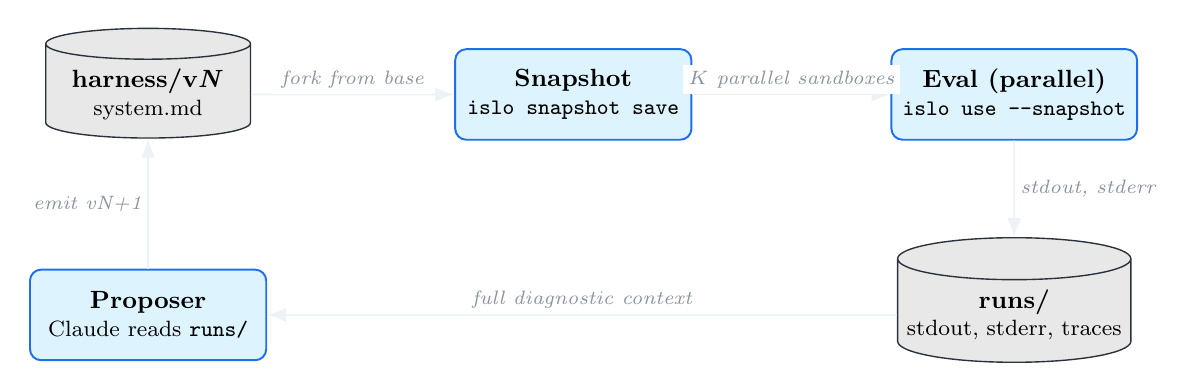
\begin{tikzpicture}[
  font=\small,
  every node/.style={align=center, font=\small},
  proc/.style={
    rectangle, rounded corners=4pt, draw=accent, line width=0.7pt,
    fill=accentlight, minimum width=3.0cm, minimum height=1.15cm, inner sep=4pt
  },
  store/.style={
    cylinder, shape border rotate=90, aspect=0.18, draw=border, line width=0.5pt,
    fill=panel!10, minimum width=2.6cm, minimum height=1.15cm
  },
  flow/.style={-{Latex[length=2.4mm]}, line width=0.6pt, draw=text!75},
  lbl/.style={font=\scriptsize\itshape, color=dim, fill=white, inner sep=2pt},
]
\node[store] (harness) at (0,0)    {\textbf{harness/v\textit{N}}\\[-1pt]\footnotesize system.md};
\node[proc]  (snap)    at (5.4,0)  {\textbf{Snapshot}\\[-1pt]\footnotesize\texttt{islo snapshot save}};
\node[proc]  (eval)    at (11.0,0) {\textbf{Eval (parallel)}\\[-1pt]\footnotesize\texttt{islo use -{}-snapshot}};
\node[proc]  (prop)    at (0,-2.8)   {\textbf{Proposer}\\[-1pt]\footnotesize Claude reads \texttt{runs/}};
\node[store] (runs)    at (11.0,-2.8){\textbf{runs/}\\[-1pt]\footnotesize stdout, stderr, traces};
\draw[flow] (harness.east) -- node[lbl,above]{fork from base}             (snap.west);
\draw[flow] (snap.east)    -- node[lbl,above]{$K$ parallel sandboxes}     (eval.west);
\draw[flow] (eval.south)   -- node[lbl,right]{stdout, stderr}             (runs.north);
\draw[flow] (runs.west)    -- node[lbl,above]{full diagnostic context}    (prop.east);
\draw[flow] (prop.north)   -- node[lbl,left]{emit v\textit{N+1}}          (harness.south);
\end{tikzpicture}
\end{center}
\newpage

% ================== Figure 2: Pass-rate bar chart ==========================
\begin{center}
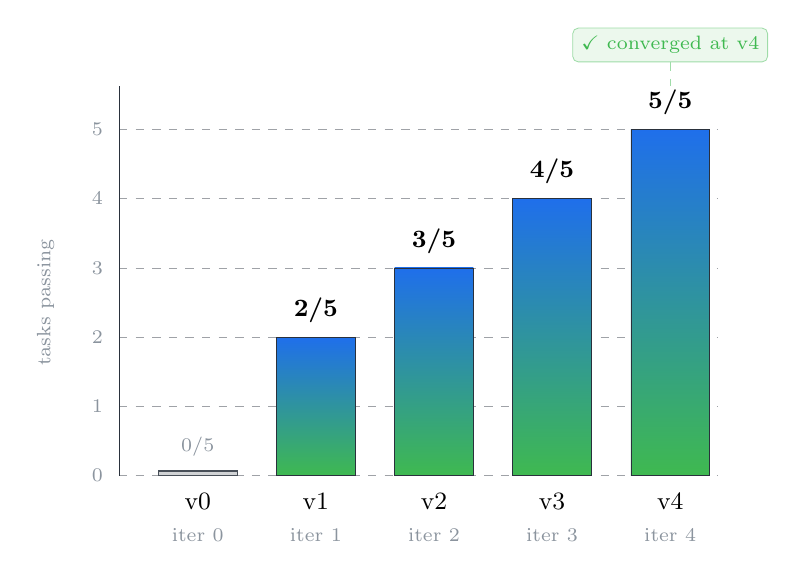
\begin{tikzpicture}[font=\small]
  \def\barW{1.0}
  \def\barGap{0.5}
  \def\maxH{4.4}
  \def\maxScore{5}
  \pgfmathsetmacro{\chartW}{4*(\barW+\barGap)+\barW}
  \draw[draw=border, line width=0.3pt] (0,0) -- (0,\maxH+0.55);
  \foreach \y in {0,1,2,3,4,5} {
    \pgfmathsetmacro{\yy}{\y/\maxScore*\maxH}
    \draw[draw=border, line width=0.2pt, dashed, opacity=0.45]
      (0,\yy) -- (\chartW+0.6,\yy);
    \node[anchor=east, font=\scriptsize\color{dim}] at (-0.08,\yy) {\y};
  }
  \node[font=\scriptsize\color{dim}, rotate=90, anchor=south] at (-0.7, \maxH/2) {tasks passing};
  \foreach \i/\h/\s [count=\xi from 0] in {0/v0/0, 1/v1/2, 2/v2/3, 3/v3/4, 4/v4/5} {
    \pgfmathsetmacro{\xpos}{0.5+\xi*(\barW+\barGap)}
    \pgfmathsetmacro{\xc}{\xpos+\barW/2}
    \pgfmathsetmacro{\hh}{\s/\maxScore*\maxH}
    \ifnum\s=0
      \draw[draw=skip, line width=0.4pt, fill=skip!25] (\xpos,0) rectangle (\xpos+\barW, 0.06);
      \node[anchor=south, font=\scriptsize\color{dim}] at (\xc, 0.12) {\s/5};
    \else
      \shade[bottom color=pass, top color=accent] (\xpos,0) rectangle (\xpos+\barW, \hh);
      \draw[draw=border, line width=0.2pt] (\xpos,0) rectangle (\xpos+\barW, \hh);
      \node[anchor=south, font=\small\bfseries] at (\xc, \hh+0.06) {\s/5};
    \fi
    \node[anchor=north, font=\small] at (\xc, -0.1) {\h};
    \node[anchor=north, font=\scriptsize\color{dim}] at (\xc, -0.55) {iter \i};
  }
  \pgfmathsetmacro{\convX}{0.5+4*(\barW+\barGap)+\barW/2}
  \node[font=\scriptsize\color{pass}, anchor=south, fill=pass!10,
        rounded corners=2pt, inner sep=3pt, draw=pass!50, line width=0.3pt]
        (cv) at (\convX, \maxH+0.85) {$\checkmark$ converged at v4};
  \draw[draw=pass!50, line width=0.3pt, dashed]
        (\convX, \maxH+0.85) -- (\convX, \maxH+0.55);
\end{tikzpicture}
\end{center}
\newpage

% ================== Figure 3: Heatmap ======================================
\begin{center}
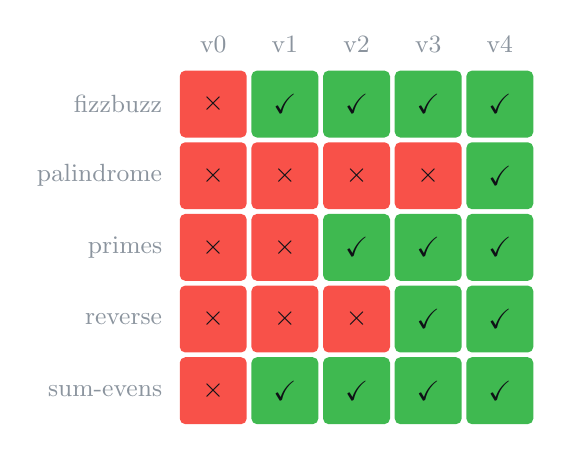
\begin{tikzpicture}[font=\small]
  \def\cell{0.85}
  \def\gap{0.06}
  \foreach \t/\name [count=\ti from 0] in {
      0/fizzbuzz, 1/palindrome, 2/primes, 3/reverse, 4/sum-evens
  } {
    \pgfmathsetmacro{\yy}{-\ti*(\cell+\gap)}
    \node[anchor=east, font=\small\color{dim}] at (-0.1, \yy-\cell/2) {\name};
  }
  \foreach \i/\h [count=\ii from 0] in {0/v0, 1/v1, 2/v2, 3/v3, 4/v4} {
    \pgfmathsetmacro{\xx}{\ii*(\cell+\gap)}
    \node[anchor=south, font=\small\color{dim}] at (\xx+\cell/2, 0.1) {\h};
  }
  \foreach \row/\col/\s in {
      0/0/0, 0/1/1, 0/2/1, 0/3/1, 0/4/1,
      1/0/0, 1/1/0, 1/2/0, 1/3/0, 1/4/1,
      2/0/0, 2/1/0, 2/2/1, 2/3/1, 2/4/1,
      3/0/0, 3/1/0, 3/2/0, 3/3/1, 3/4/1,
      4/0/0, 4/1/1, 4/2/1, 4/3/1, 4/4/1
  } {
    \pgfmathsetmacro{\xx}{\col*(\cell+\gap)}
    \pgfmathsetmacro{\yy}{-\row*(\cell+\gap)}
    \ifnum\s=1
      \fill[pass, rounded corners=2pt] (\xx,\yy) rectangle (\xx+\cell, \yy-\cell);
      \node[font=\bfseries, color=bg] at (\xx+\cell/2, \yy-\cell/2) {$\checkmark$};
    \else
      \fill[fail, rounded corners=2pt] (\xx,\yy) rectangle (\xx+\cell, \yy-\cell);
      \node[font=\bfseries, color=bg] at (\xx+\cell/2, \yy-\cell/2) {$\times$};
    \fi
  }
\end{tikzpicture}
\end{center}
\newpage

% ================== Figure 4: Dashboard layout sketch ======================
\newgeometry{paperwidth=18cm, paperheight=12cm, margin=4mm}
\begin{center}
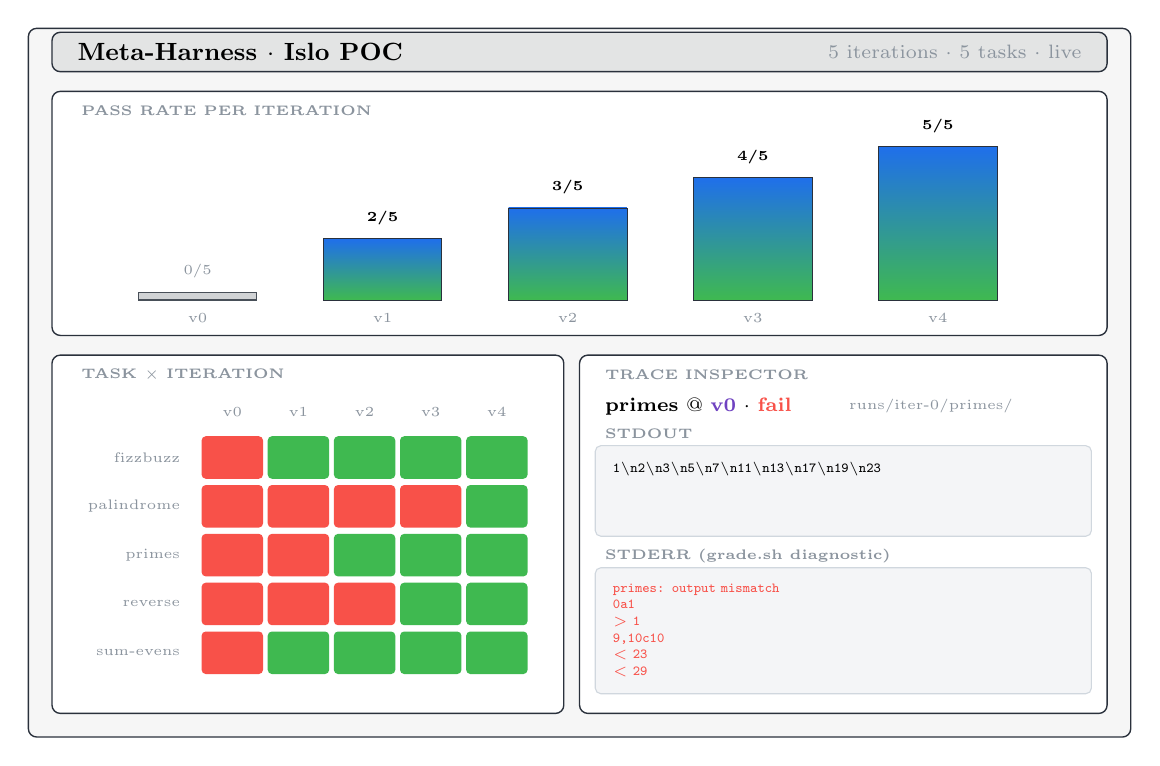
\begin{tikzpicture}[
  font=\scriptsize,
  panel/.style={rectangle, rounded corners=3pt, draw=border, fill=white, line width=0.5pt},
  hdr/.style={rectangle, rounded corners=3pt, draw=border, fill=panel!12, line width=0.5pt},
  sectlbl/.style={font=\tiny\bfseries, color=dim, anchor=west}
]
  \draw[panel, fill=panel!4] (0,0) rectangle (14,9);
  \draw[hdr] (0.30,8.45) rectangle (13.70,8.95);
  \node[anchor=west, font=\small\bfseries] at (0.50,8.70) {Meta-Harness $\cdot$ Islo POC};
  \node[anchor=east, color=dim] at (13.50,8.70) {5 iterations $\cdot$ 5 tasks $\cdot$ live};
  \draw[panel] (0.30,5.10) rectangle (13.70,8.20);
  \node[sectlbl] at (0.55,7.95) {PASS RATE PER ITERATION};
  \foreach \i/\score in {0/0, 1/2, 2/3, 3/4, 4/5} {
    \pgfmathsetmacro{\xL}{1.40+\i*2.35}
    \pgfmathsetmacro{\xC}{\xL+0.75}
    \pgfmathsetmacro{\h}{\score/5*1.95}
    \ifnum\score=0
      \draw[draw=skip, fill=skip!25] (\xL,5.55) rectangle (\xL+1.50,5.65);
      \node[anchor=south, font=\tiny, color=dim] at (\xC,5.70) {0/5};
    \else
      \shade[bottom color=pass, top color=accent] (\xL,5.55) rectangle (\xL+1.50,5.55+\h);
      \draw[draw=border, line width=0.2pt] (\xL,5.55) rectangle (\xL+1.50,5.55+\h);
      \node[anchor=south, font=\tiny\bfseries] at (\xC,5.55+\h+0.05) {\score/5};
    \fi
    \node[anchor=north, font=\tiny, color=dim] at (\xC,5.50) {v\i};
  }
  \draw[panel] (0.30,0.30) rectangle (6.80,4.85);
  \node[sectlbl] at (0.55,4.60) {TASK $\times$ ITERATION};
  \foreach \name [count=\r from 0] in {fizzbuzz,palindrome,primes,reverse,sum-evens} {
    \pgfmathsetmacro{\yy}{3.55-\r*0.62}
    \node[anchor=east, font=\tiny, color=dim] at (2.05,\yy) {\name};
  }
  \foreach \i in {0,1,2,3,4} {
    \pgfmathsetmacro{\xC}{2.20+\i*0.84+0.39}
    \node[anchor=south, font=\tiny, color=dim] at (\xC,3.95) {v\i};
  }
  \foreach \row/\col/\s in {
      0/0/0, 0/1/1, 0/2/1, 0/3/1, 0/4/1,
      1/0/0, 1/1/0, 1/2/0, 1/3/0, 1/4/1,
      2/0/0, 2/1/0, 2/2/1, 2/3/1, 2/4/1,
      3/0/0, 3/1/0, 3/2/0, 3/3/1, 3/4/1,
      4/0/0, 4/1/1, 4/2/1, 4/3/1, 4/4/1
  } {
    \pgfmathsetmacro{\xL}{2.20+\col*0.84}
    \pgfmathsetmacro{\yC}{3.55-\row*0.62}
    \ifnum\s=1
      \fill[pass, rounded corners=1.5pt] (\xL,\yC-0.27) rectangle (\xL+0.78,\yC+0.27);
    \else
      \fill[fail, rounded corners=1.5pt] (\xL,\yC-0.27) rectangle (\xL+0.78,\yC+0.27);
    \fi
  }
  \draw[panel] (7.00,0.30) rectangle (13.70,4.85);
  \node[sectlbl] at (7.20,4.60) {TRACE INSPECTOR};
  \node[anchor=west, font=\scriptsize] at (7.20,4.20)
    {\textbf{primes} @ \textcolor{accent2}{\textbf{v0}} $\cdot$ \textcolor{fail}{\textbf{fail}}};
  \node[anchor=west, font=\tiny, color=dim] at (10.30,4.20) {runs/iter-0/primes/};
  \node[sectlbl] at (7.20,3.85) {STDOUT};
  \draw[draw=codeborder, fill=codebg, rounded corners=2pt]
    (7.20,2.55) rectangle (13.50,3.70);
  \node[anchor=north west, font=\ttfamily\tiny, color=black, text width=6.05cm] at (7.30,3.62)
    {1\textbackslash n2\textbackslash n3\textbackslash n5\textbackslash n7\textbackslash n11\textbackslash n13\textbackslash n17\textbackslash n19\textbackslash n23};
  \node[sectlbl] at (7.20,2.30) {STDERR (grade.sh diagnostic)};
  \draw[draw=codeborder, fill=codebg, rounded corners=2pt]
    (7.20,0.55) rectangle (13.50,2.15);
  \node[anchor=north west, font=\ttfamily\tiny, color=fail, text width=6.05cm] at (7.30,2.07)
    {primes: output mismatch\\
     0a1\\
     \textgreater{} 1\\
     9,10c10\\
     \textless{} 23\\
     \textless{} 29};
\end{tikzpicture}
\end{center}

\end{document}
